\documentclass{article}
\usepackage[utf8]{inputenc}
\usepackage{amsmath}
\usepackage{amsfonts}
\usepackage[a4paper, margin=1in]{geometry}
\usepackage{graphicx}
\usepackage{enumitem}
\usepackage{listings}
\usepackage{xcolor}
\title{Mid Term Exam 1}
\author{Steve Gillet}
\date{\today}

% Custom information
\newcommand{\className}{Course: Linear Control Design – ASEN 5014-001 – Fall 2024}
\newcommand{\professorName}{Professor: Dale Lawrence}
\newcommand{\taName}{Teaching Assistant: Karan Muvvala}

\lstdefinestyle{pythonstyle}{
    language=Python,
    basicstyle=\ttfamily\footnotesize\color{white},
    keywordstyle=\bfseries\color{yellow},
    commentstyle=\itshape\color{gray},
    stringstyle=\color{orange},
    showstringspaces=false,
    numberstyle=\tiny\color{pink},
    numbersep=5pt,
    frame=single,
    breaklines=true,
    backgroundcolor=\color{black},
}

\begin{document}

% Title
\maketitle
\begin{center}
    \large{\className} \\
    \large{\professorName} \\
    \large{\taName}
\end{center}

\section*{Question 1}

For each of the following statements, either show why it is true, or fix it to make it true and provide a corresponding explanation why.

\subsection*{(a) \[\text{span}\left\{ \begin{bmatrix} 1 \\ 1 \\ 1 \end{bmatrix}, \begin{bmatrix} 0 \\ 1 \\ 0 \end{bmatrix}, \begin{bmatrix} 1 \\ 1 \\ 1 \end{bmatrix} \right\} = 2 \]}

The span of the set of vectors is $2$ because although there are $3$ vectors, one of them is a linear combination of the other two. Therefore, there are only two linearly independent vectors, making the dimension of the span equal to two.

To show that the third vector can be obtained by adding the first and second vectors, we consider the given vectors:

\[\mathbf{v}_3 = \mathbf{v}_1 + \mathbf{v}_2 = \begin{bmatrix} 1 \\ 0 \\ 1 \end{bmatrix} + \begin{bmatrix} 0 \\ 1 \\ 0 \end{bmatrix} = \begin{bmatrix} 1 \\ 1 \\ 1 \end{bmatrix}\]

This shows that $\mathbf{v}_3$ is a linear combination of $\mathbf{v}_1$ and $\mathbf{v}_2$, meaning it does not contribute any additional dimension to the span. Therefore, the set of vectors has only two linearly independent vectors, and the span is of dimension $2$.

\subsection*{(b) A basis for $\mathbf{R}^3$ is:
\[ \left\{ \begin{bmatrix} 1 \\ 1 \end{bmatrix}, \begin{bmatrix} 0 \\ 2 \end{bmatrix}, \begin{bmatrix} -1 \\ 0 \end{bmatrix} \right\} \]
}

Despite the fact that there are three vectors, each vector only has two elements, and therefore they couldn't possibly span three dimensions. A two-element vector can only describe two dimensions, which means one of the vectors is superfluous in this case. However, if you expanded the vectors by adding a third element, say a $0$ to the first two and a $1$ to the last one, then you would have three linearly independent three-dimensional vectors that could span $\mathbb{R}^3$, thus forming a basis for $\mathbb{R}^3$.

\subsection*{(c) The set
\[
\left\{ 
\begin{bmatrix} 1 \\ 0 \\ 0 \\ 1 \end{bmatrix}, 
\begin{bmatrix} 0 \\ 0 \\ 1 \\ 0 \end{bmatrix}, 
\begin{bmatrix} 1 \\ 0 \\ 1 \\ 0 \end{bmatrix}, 
\begin{bmatrix} 1 \\ 0 \\ 1 \\ 1 \end{bmatrix} 
\right\}
\]
cannot be a spanning set because it is linearly dependent.}


This statement is true. The given set cannot be a spanning set because none of the vectors have an element in the second position, which means they cannot fully represent all four dimensions of the space. Additionally, the fourth vector is a linear combination of the first two vectors.

To illustrate this, consider the following vectors:

\[
\mathbf{v}_1 = \begin{bmatrix} 1 \\ 0 \\ 0 \\ 1 \end{bmatrix}, \quad 
\mathbf{v}_2 = \begin{bmatrix} 0 \\ 0 \\ 1 \\ 0 \end{bmatrix}, \quad 
\mathbf{v}_4 = \begin{bmatrix} 1 \\ 0 \\ 1 \\ 1 \end{bmatrix}
\]

Notice that:

\[
\mathbf{v}_4 = \mathbf{v}_1 + \mathbf{v}_2 = \begin{bmatrix} 1 \\ 0 \\ 0 \\ 1 \end{bmatrix} + \begin{bmatrix} 0 \\ 0 \\ 1 \\ 0 \end{bmatrix} = \begin{bmatrix} 1 \\ 0 \\ 1 \\ 1 \end{bmatrix}
\]

This shows that $\mathbf{v}_4$ is a linear combination of $\mathbf{v}_1$ and $\mathbf{v}_2$, making the set linearly dependent. Therefore, it cannot span the entire space.

\subsection*{(d) For any vector space $V$, there can be only one minimal spanning set.}


This statement is false. There can be infinitely many minimal spanning sets. For example, for a vector space in $\mathbb{R}^3$, there could be a minimal spanning set:

\[
\left\{ 
\begin{bmatrix} 1 \\ 0 \\ 0 \end{bmatrix}, 
\begin{bmatrix} 0 \\ 1 \\ 0 \end{bmatrix}, 
\begin{bmatrix} 0 \\ 0 \\ 1 \end{bmatrix} 
\right\}
\]

or

\[
\left\{ 
\begin{bmatrix} 0.5 \\ 0 \\ 0 \end{bmatrix}, 
\begin{bmatrix} 0 \\ 0.5 \\ 0 \end{bmatrix}, 
\begin{bmatrix} 0 \\ 0 \\ 0.5 \end{bmatrix} 
\right\}
\]

or even

\[
\left\{ 
\begin{bmatrix} 1 \\ 2 \\ 3 \end{bmatrix}, 
\begin{bmatrix} 3 \\ 2 \\ 1 \end{bmatrix}, 
\begin{bmatrix} 2 \\ 3 \\ 1 \end{bmatrix} 
\right\}
\]

All of these sets are minimal spanning sets (i.e., bases) for $\mathbb{R}^3$. The elements of each set are linearly independent and span the vector space, but there are infinitely many different sets that can serve as a basis for the same vector space.

\subsection*{(e) A linear equation $y = Mx$ has unique solutions if and only if $y \in CS(M)$.}

This statement is false. The equation $y = Mx$ has solutions if and only if $y$ is in the column space of $M$. However, these solutions are unique if and only if the right null space of $M$ is trivial (i.e., consists only of the zero vector). If the right null space is non-trivial, then there are infinitely many solutions since there are non-zero vectors in the null space that can be added to a particular solution to generate other solutions.

\subsection*{(f): A linear equation \(y = Mx\) fails to have a solution iff \(RN(M)\) is non-trivial.}
This statement is false. The equation $y = Mx$ fails to have a solution if $y$ is not in the column space of $M$. If the right null space of $M$ is non-trivial, it means that $y = Mx$ has multiple solutions, not that it fails to have a solution. Again because of the non-zero vectors in the null space that can be added to a solution to produce more solutions.

\subsection*{(g) span\(\left\{ 
    \begin{bmatrix} 
    1 \\ -1 \\ 3 \\ 0 \\ 5 
    \end{bmatrix}, 
    \begin{bmatrix} 
    2 \\ 1 \\ 2 \\ 4 \\ -6 
    \end{bmatrix}, 
    \begin{bmatrix} 
    1 \\ 2 \\ -1 \\ 4 \\ 1 
    \end{bmatrix} 
    \right\} > \text{span}\left\{
    \begin{bmatrix} 
    1 \\ 0 \\ 0 
    \end{bmatrix}, 
    \begin{bmatrix} 
    1 \\ 2 \\ 0 
    \end{bmatrix}, 
    \begin{bmatrix} 
    -1 \\ 0 \\ 1 
    \end{bmatrix} 
    \right\}\)}


This statement is true. The span of the first set is $3$ since there are $3$ linearly independent vectors, while the span of the second set is $2$ because there are only two independent vectors. The first vector in the second set is a linear combination of the second and third vectors, which can be shown as follows:

Consider the vectors:

\[
\mathbf{v}_1 = \begin{bmatrix} 1 \\ 1 \end{bmatrix}, \quad 
\mathbf{v}_2 = \begin{bmatrix} 0 \\ 2 \end{bmatrix}, \quad 
\mathbf{v}_3 = \begin{bmatrix} -1 \\ 0 \end{bmatrix}
\]

We can express $\mathbf{v}_1$ as a linear combination of $\mathbf{v}_2$ and $\mathbf{v}_3$:

\[
\mathbf{v}_1 = a \cdot \mathbf{v}_2 + b \cdot \mathbf{v}_3 = a \begin{bmatrix} 0 \\ 2 \end{bmatrix} + b \begin{bmatrix} -1 \\ 0 \end{bmatrix}
\]

To satisfy $\mathbf{v}_1 = \begin{bmatrix} 1 \\ 1 \end{bmatrix}$, we solve the following system of equations:

\[
- b = 1 \\ 
2a = 1
\]

From this, we find $a = \frac{1}{2}$ and $b = -1$. Therefore:

\[
\mathbf{v}_1 = \frac{1}{2} \begin{bmatrix} 0 \\ 2 \end{bmatrix} + (-1) \begin{bmatrix} -1 \\ 0 \end{bmatrix} = \begin{bmatrix} 1 \\ 1 \end{bmatrix}
\]

This shows that $\mathbf{v}_1$ is a linear combination of $\mathbf{v}_2$ and $\mathbf{v}_3$, indicating that the set is linearly dependent. In a set of vectors with two elements, there can only be two linearly independent vectors at most.

\subsection*{(h) \text{span}\(\left\{ 
    \begin{bmatrix} 
    1 \\ 0 \\ 0 \\ 1
    \end{bmatrix}
    \begin{bmatrix}
    0 \\ 0 \\ 1 \\ 0
    \end{bmatrix}
    \begin{bmatrix}
    1 \\ 1 \\ 1 \\ 0 
    \end{bmatrix}
    \right\} 
    = \text{span}\left\{ 
    \begin{bmatrix} 
    1 \\ 0 \\ 1 
    \end{bmatrix}, 
    \begin{bmatrix} 
    0 \\ 1 \\ 0 
    \end{bmatrix}, 
    \begin{bmatrix} 
    1 \\ 1 \\ 1 
    \end{bmatrix}
    \right\}\).
}

The statement is false. The span of the first set 
\[
\left\{ 
\begin{bmatrix} 
1 \\ 0 \\ 0 \\ 1 
\end{bmatrix}, 
\begin{bmatrix} 
0 \\ 0 \\ 1 \\ 0 
\end{bmatrix}, 
\begin{bmatrix} 
1 \\ 1 \\ 1 \\ 0 
\end{bmatrix}
\right\}
\]
is 3 because these three vectors are linearly independent.

The span of the second set 
\[
\left\{ 
\begin{bmatrix} 
1 \\ 0 \\ 1 
\end{bmatrix}, 
\begin{bmatrix} 
0 \\ 1 \\ 0 
\end{bmatrix}, 
\begin{bmatrix} 
1 \\ 1 \\ 1 
\end{bmatrix}
\right\}
\]
is 2 because the first two vectors are linearly independent, but the third vector is a linear combination of the first two.

To show this, notice that:
\[
\begin{bmatrix} 
1 \\ 1 \\ 1 
\end{bmatrix} 
= \begin{bmatrix} 
1 \\ 0 \\ 1 
\end{bmatrix} + \begin{bmatrix} 
0 \\ 1 \\ 0 
\end{bmatrix}.
\]

Thus, the third vector in the second set is dependent on the first two, reducing the dimension of the span to 2.

You could make the statement true by changing the third vector in the second set to something linearly independent of the first two, like 
\[
\begin{bmatrix} 
2 \\ 1 \\ 1 
\end{bmatrix}.
\]

\subsection*{(i) The RS(M) is always non-trivial.}

The statement is false. The row space of a matrix \( M \), denoted as \( \text{RS}(M) \), is not always non-trivial. The row space can be trivial (i.e., consist only of the zero vector) if \( M \) is a zero matrix. For example, if \( M \) is the zero matrix:

\[
M = \begin{bmatrix} 
0 & 0 \\
0 & 0
\end{bmatrix},
\]

then \( \text{RS}(M) = \{ \mathbf{0} \} \), which is trivial.

To fix the statement, it could be revised to say:
"The row space of a non-zero matrix is always non-trivial."

This is true because a non-zero matrix has at least one non-zero row, so the row space will contain non-zero vectors.

\subsection*{(j) If a mapping is onto, then \( M \) has linearly independent columns.}

The statement is false. If a mapping is onto, this implies that the row space of the matrix spans the entire codomain, but it does not necessarily mean that the columns of the matrix are linearly independent. For example, a \( 3 \times 2 \) matrix can map onto \( \mathbb{R}^3 \), but the columns may still be linearly dependent. Consider:

\[
M = \begin{bmatrix} 
1 & 2 \\
1 & 2 \\
1 & 2
\end{bmatrix}.
\]

Here, the matrix is onto (it maps onto \( \mathbb{R}^3 \)), but the columns are linearly dependent because one column is a scalar multiple of the other.

To fix the statement, it could be revised to:
"If a mapping is one-to-one, then \( M \) has linearly independent columns."

This is true because injectivity implies that no column of the matrix can be written as a linear combination of the others, which means the columns are linearly independent.

\section*{Question 2. Given the basis sets B and C below}

\begin{enumerate}[label={\alph*.}]
    \item Find the coordinate representation of 
    \[
    z^T = [18 \quad 2.6 \quad 3.1 \quad 3.0 \quad 34 \quad 7.1]
    \]
    in each basis.
    \item Determine if \( w \) given below lies in \( \text{span}(B) \).
    \[
    w^T = [3 \quad 24 \quad 3 \quad -12 \quad 1 \quad 6]
    \]
    \item Find an orthonormal basis for \( \text{span}(B) \). Is this also an orthonormal basis for \( \text{span}(C) \)
\end{enumerate}

The basis sets \( B \) and \( C \) are given by:

\[
B = \left\{
\begin{bmatrix} 
3 & 1 & 2 \\
1 & 1 & 0 \\
-1 & 2 & 3 \\
2 & -1 & -2 \\
4 & -2 & 4 \\
2 & 3 & 1 
\end{bmatrix}
\right\}, 
\quad C = \left\{
\begin{bmatrix} 
5 & 2 & 0 \\
1 & 0 & 2 \\
2 & -3 & 1 \\
0 & 3 & 0 \\
8 & 6 & -8 \\
3 & -1 & 5 
\end{bmatrix}
\right\}.
\]

\subsection*{(a)}

To find the coordinate representation of \( z^T = [18 \quad 2.6 \quad 3.1 \quad 3.0 \quad 34 \quad 7.1] \) in each basis, we need to solve the following system of equations for each basis:

For basis \( B \), we solve for \( c_1, c_2, c_3 \) in the equation:

\[
B \cdot \begin{bmatrix} c_1 \\ c_2 \\ c_3 \end{bmatrix} = z^T.
\]

This gives the following system of equations:

\[
\begin{aligned}
3c_1 + 1c_2 + 2c_3 &= 18 \\
1c_1 + 1c_2 + 0c_3 &= 2.6 \\
-1c_1 + 2c_2 + 3c_3 &= 3.1 \\
2c_1 - 1c_2 - 2c_3 &= 3.0 \\
4c_1 - 2c_2 + 4c_3 &= 34 \\
2c_1 + 3c_2 + 1c_3 &= 7.1
\end{aligned}
\]

For basis \( C \), we solve for \( d_1, d_2, d_3 \) in the equation:

\[
C \cdot \begin{bmatrix} d_1 \\ d_2 \\ d_3 \end{bmatrix} = z^T.
\]

This gives the following system of equations:

\[
\begin{aligned}
5d_1 + 2d_2 + 0d_3 &= 18 \\
1d_1 + 0d_2 + 2d_3 &= 2.6 \\
2d_1 - 3d_2 + 1d_3 &= 3.1 \\
0d_1 + 3d_2 + 0d_3 &= 3.0 \\
8d_1 + 6d_2 - 8d_3 &= 34 \\
3d_1 - 1d_2 + 5d_3 &= 7.1
\end{aligned}
\]

The coordinate representation of \( z^T = [18 \quad 2.6 \quad 3.1 \quad 3.0 \quad 34 \quad 7.1] \) in each basis is as follows:

- In the basis \( B \), the coordinates are approximately:
\[
[4.2, -1.6, 3.5]
\]

- In the basis \( C \), the coordinates are approximately:
\[
[3.2, 1.0, -0.3]
\]

\subsection*{b. Determine if \( w \) given below lies in \( \text{span}(B) \).}

To determine if \( w^T = [3 \quad 24 \quad 3 \quad -12 \quad 1 \quad 6] \) lies in \( \text{span}(B) \), we need to check if \( w \) can be written as a linear combination of the columns of \( B \).

This requires solving the system:
\[
B \cdot \begin{bmatrix} c_1 \\ c_2 \\ c_3 \end{bmatrix} = w^T.
\]

The system is:
\[
\begin{aligned}
3c_1 + 1c_2 + 2c_3 &= 3 \\
1c_1 + 1c_2 + 0c_3 &= 24 \\
-1c_1 + 2c_2 + 3c_3 &= 3 \\
2c_1 - 1c_2 - 2c_3 &= -12 \\
4c_1 - 2c_2 + 4c_3 &= 1 \\
2c_1 + 3c_2 + 1c_3 &= 6
\end{aligned}
\]

Solving this system, we find that there is no solution. Thus, \( w \) does not lie in \( \text{span}(B) \).

\subsection*{c. Find an orthonormal basis for \( \text{span}(B) \). Is this also an orthonormal basis for \( \text{span}(C) \)?}

To find the orthonormal basis for B and C we perform QR decomposition (Gram-Schmidt process) on both matrices \( B \) and \( C \) to find their orthonormal bases. The orthonormal basis for each matrix is given by the columns of the \( Q \) matrix from the decomposition.

The orthonormal basis for \( \text{span}(B) \) is:

\[
Q_B = \begin{bmatrix}
-0.507 & -0.263 & -0.039 \\
-0.169 & -0.237 & 0.164 \\
0.169 & -0.436 & -0.593 \\
-0.338 & 0.199 & 0.553 \\
-0.676 & 0.397 & -0.529 \\
-0.338 & -0.698 & 0.185
\end{bmatrix}
\]

The orthonormal basis for \( \text{span}(C) \) is:

\[
Q_C = \begin{bmatrix}
-0.493 & -0.063 & 0.284 \\
-0.099 & -0.080 & 0.309 \\
-0.197 & -0.661 & -0.306 \\
0 & 0.502 & 0.455 \\
-0.788 & 0.367 & -0.372 \\
-0.296 & -0.406 & 0.620
\end{bmatrix}
\]

As we can see, the orthonormal bases for \( \text{span}(B) \) and \( \text{span}(C) \) are different. Therefore, the orthonormal basis for \( \text{span}(B) \) is not the same as the orthonormal basis for \( \text{span}(C) \).

\section*{Question 3. For the following differential equation}

\[
\dddot{y}(t) - 3\ddot{y}(t) + 2y(t) = \ddot{u}(t) - 3\dot{u}(t)
\]

\subsection*{a. Find the transfer function relating \( u(s) \) and \( y(s) \).}

Taking the Laplace transform of both sides of the differential equation and assuming zero initial conditions:

\[
s^3 Y(s) - 3s^2 Y(s) + 2 Y(s) = s^2 U(s) - 3s U(s)
\]

We factor the equation:

\[
(s^3 - 3s^2 + 2) Y(s) = (s^2 - 3s) U(s)
\]

The transfer function is then:

\[
\frac{Y(s)}{U(s)} = \frac{s^2 - 3s}{s^3 - 3s^2 + 2}
\]

\subsection*{b. Find a state-space model in the controllable canonical form.}

To convert the transfer function into state-space form, we define the state variables:

\[
x_1 = y(t), \quad x_2 = \dot{y}(t), \quad x_3 = \ddot{y}(t)
\]

Then, the system of equations becomes:

\[
\dot{x}_1 = x_2
\]
\[
\dot{x}_2 = x_3
\]
\[
\dot{x}_3 = -2x_1 + 3x_3 + \ddot{u}(t) - 3\dot{u}(t)
\]

In matrix form, the state-space representation in controllable canonical form is:

\[
\begin{bmatrix}
\dot{x}_1 \\
\dot{x}_2 \\
\dot{x}_3
\end{bmatrix}
=
\begin{bmatrix}
0 & 1 & 0 \\
0 & 0 & 1 \\
-2 & 0 & 3
\end{bmatrix}
\begin{bmatrix}
x_1 \\
x_2 \\
x_3
\end{bmatrix}
+
\begin{bmatrix}
0 \\
0 \\
1
\end{bmatrix}
\ddot{u}(t) + 
\begin{bmatrix}
0 \\
0 \\
-3
\end{bmatrix} \dot{u}(t)
\]

The output equation is:

\[
y(t) = \begin{bmatrix} 1 & 0 & 0 \end{bmatrix} \begin{bmatrix} x_1 \\ x_2 \\ x_3 \end{bmatrix}
\]

\subsection*{c. Draw a simulation diagram and label the state variables on the diagram.}

\begin{figure}[h!]
    \centering
    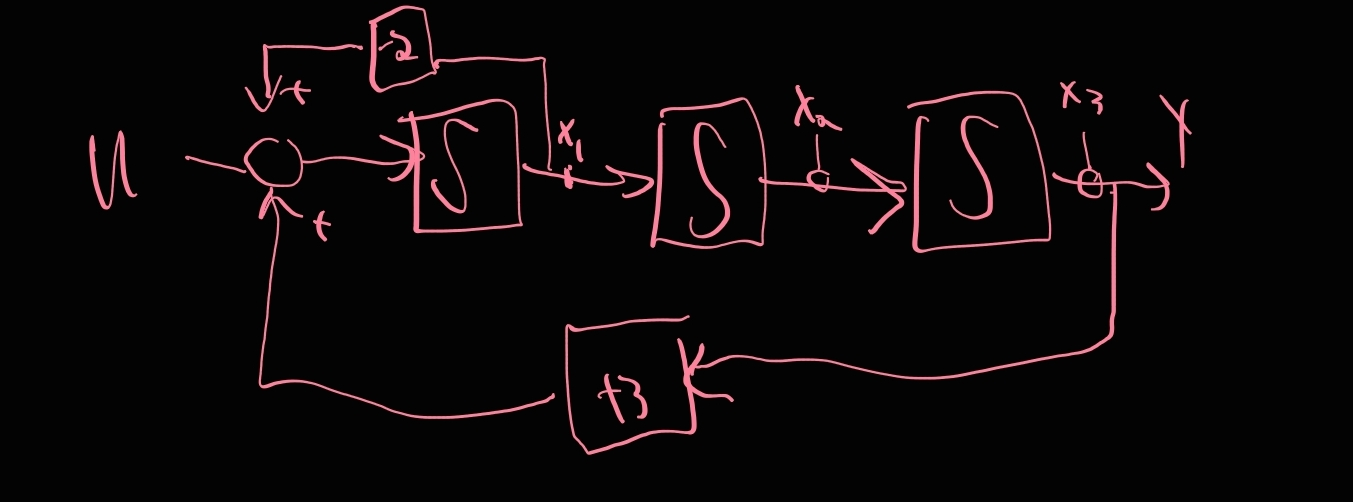
\includegraphics[width=0.7\textwidth]{midterm3c.jpg}
    \caption{Simulation diagram for the system described in part (c).}
    \label{fig:midterm3c}
\end{figure}

\section*{Question 4. Show whether or not the set of positive real numbers \( \mathbb{R}^+ \) is a vector space over \( \mathbb{R} \), i.e., \( V = (G,F) = (\mathbb{R}^+, \mathbb{R}) \) under the following operations:}

The operations are defined as follows:

- Group operator "+" (vector addition) is defined by:
\[
x " + " y = x \cdot y
\]
where \( x, y \in \mathbb{R}^+ \) and \( \cdot \) is the usual multiplication of real numbers.

- Scalar multiplication "·" is defined by:
\[
c " \cdot " x = x^c
\]
for \( x \in \mathbb{R}^+ \) and \( c \in \mathbb{R} \), where \( x^c \) is the usual exponentiation.

\subsection*{Conditions for a Vector Space:}

To determine if \( \mathbb{R}^+ \) with these operations forms a vector space, we must check the 10 axioms for vector spaces. A vector space must satisfy the following properties:

1. Closure under addition: For all \( x, y \in \mathbb{R}^+ \), is \( x " + " y \in \mathbb{R}^+ \)?
   \[
   x " + " y = x \cdot y \in \mathbb{R}^+ \quad \text{(Yes, since the product of two positive real numbers is still positive).}
   \]

2. Commutativity of addition: Is \( x " + " y = y " + " x \)?
   \[
   x " + " y = x \cdot y = y \cdot x = y " + " x \quad \text{(Yes, multiplication is commutative).}
   \]

3. Associativity of addition: Is \( (x " + " y) " + " z = x " + " (y " + " z) \)?
   \[
   (x " + " y) " + " z = (x \cdot y) \cdot z = x \cdot (y \cdot z) = x " + " (y " + " z) \quad \text{(Yes, multiplication is associative).}
   \]

4. Existence of an additive identity: Is there an element \( 0 \in \mathbb{R}^+ \) such that \( x " + " 0 = x \)?
   \[
   x " + " 1 = x \cdot 1 = x \quad \text{(Yes, 1 is the additive identity).}
   \]

5. Existence of additive inverses: For each \( x \in \mathbb{R}^+ \), does there exist an element \( -x \in \mathbb{R}^+ \) such that \( x " + " (-x) = 0 \)?
   \[
   x " + " y = x \cdot y = 1 \quad \text{(The inverse of \( x \) is \( \frac{1}{x} \), which is in \( \mathbb{R}^+ \), so this is satisfied).}
   \]

6. Closure under scalar multiplication: For all \( c \in \mathbb{R} \) and \( x \in \mathbb{R}^+ \), is \( c " \cdot " x \in \mathbb{R}^+ \)?
   \[
   c " \cdot " x = x^c \quad \text{(This is satisfied, since exponentiation of positive real numbers is defined for all real scalars \( c \)).}
   \]

7. Distributivity of scalar multiplication with respect to vector addition: Is \( c " \cdot " (x " + " y) = (c " \cdot " x) " + " (c " \cdot " y) \)?
   \[
   c " \cdot " (x " + " y) = (x \cdot y)^c = x^c \cdot y^c = (c " \cdot " x) " + " (c " \cdot " y) \quad \text{(Yes, by exponentiation rules).}
   \]

8. Distributivity of scalar multiplication with respect to scalar addition: Is \( (c + d) " \cdot " x = (c " \cdot " x) " + " (d " \cdot " x) \)?
   \[
   (c + d) " \cdot " x = x^{c+d} = x^c \cdot x^d = (c " \cdot " x) " + " (d " \cdot " x) \quad \text{(Yes, by exponentiation rules).}
   \]

9. Associativity of scalar multiplication: Is \( c " \cdot " (d " \cdot " x) = (cd) " \cdot " x \)?
   \[
   c " \cdot " (d " \cdot " x) = c " \cdot " (x^d) = (x^d)^c = x^{cd} = (cd) " \cdot " x \quad \text{(Yes, by exponentiation rules).}
   \]

10. Existence of a scalar identity: Is \( 1 " \cdot " x = x \)?
   \[
   1 " \cdot " x = x^1 = x \quad \text{(Yes, by definition of exponentiation).}
   \]

\subsection*{Conclusion:}

Since all 10 axioms for a vector space are satisfied, the set of positive real numbers \( \mathbb{R}^+ \) with the defined operations forms a vector space over \( \mathbb{R} \).

\section*{Honor Code}

\begin{figure}[h!]
    \centering
    
\includegraphics[width=0.7\textwidth]{midtermHonorCode.jpg}
    \caption{Signed Honor Code}
    \label{fig:midtermHonorCode}
\end{figure}

\section*{Code}

Below is the python code I used in the midterm for calculations.

\subsection*{Question 1 Part g}
\begin{lstlisting}[style=pythonstyle]
import numpy as np

# Define the matrix of vectors
A = np.array([
    [1, 2, 1],
    [-1, 1, 2],
    [3, 2, -1],
    [0, 4, 4],
    [5, -6, 1]
])

# Perform QR decomposition
Q, R = np.linalg.qr(A)

# Check the rank of the R matrix
rank = np.sum(np.abs(np.diag(R)) > 1e-10)

print(R)

# Determine linear independence
if rank == A.shape[1]:
    print("The set of vectors is linearly independent.")
else:
    print("The set of vectors is linearly dependent.")
\end{lstlisting}
    
\subsection*{Question 1 Part h}
\begin{lstlisting}[style=pythonstyle]
import numpy as np
from numpy.linalg import qr

# Matrix from the first span set
A = np.array([[1, 0, 1],
                [0, 0, 1],
                [0, 1, 1],
                [1, 0, 0]])

print(A)

# Perform QR decomposition
Q, R = qr(A)

# Check linear independence: If R has any zero diagonal entries, the columns are linearly dependent.
independent = np.all(np.abs(np.diag(R)) > 1e-10)

print(R)

if independent:
    print("The vectors are linearly independent.")
else:
    print("The vectors are linearly dependent.")

# Matrix from the second span set
A = np.array([[1, 0, 1],
                [0, 1, 1],
                [1, 0, 1]])

print(A)

# Perform QR decomposition
Q, R = qr(A)

# Check linear independence: If R has any zero diagonal entries, the columns are linearly dependent.
independent = np.all(np.abs(np.diag(R)) > 1e-10)

print(R)

if independent:
    print("The vectors are linearly independent.")
else:
    print("The vectors are linearly dependent.")
    
\end{lstlisting}

\subsection*{Question 2 Part a}
\begin{lstlisting}[style=pythonstyle]
import numpy as np

# Define the matrix B
B = np.array([[3, 1, 2],
                [1, 1, 0],
                [-1, 2, 3],
                [2, -1, -2],
                [4, -2, 4],
                [2, 3, 1]])

# Define the matrix C
C = np.array([[5, 2, 0],
                [1, 0, 2],
                [2, -3, 1],
                [0, 3, 0],
                [8, 6, -8],
                [3, -1, 5]])

# Define the vector z
z = np.array([18, 2.6, 3.1, 3.0, 34, 7.1])

# Solve for the coordinates in the basis B
coordinates_B = np.linalg.lstsq(B, z, rcond=None)[0]

# Solve for the coordinates in the basis C
coordinates_C = np.linalg.lstsq(C, z, rcond=None)[0]

print(coordinates_B, coordinates_C)
    
\end{lstlisting}

\subsection*{Question 2 Part b}
\begin{lstlisting}[style=pythonstyle]
import numpy as np

# Define matrix B again
B = np.array([[3, 1, 2],
                [1, 1, 0],
                [-1, 2, 3],
                [2, -1, -2],
                [4, -2, 4],
                [2, 3, 1]])

# Define the vector w
w = np.array([3, 24, 3, -12, 1, 6])

# Solve the system B * [c1, c2, c3] = w
# We can use np.linalg.lstsq to see if there is a solution
solution, residuals, rank, s = np.linalg.lstsq(B, w, rcond=None)

# Check if there are any non-zero residuals (indicating no exact solution)
print(solution, residuals)        
\end{lstlisting}

\subsection*{Question 2 Part c}
\begin{lstlisting}[style=pythonstyle]
import numpy as np
from numpy.linalg import qr

# Define matrix B
B = np.array([[3, 1, 2],
                [1, 1, 0],
                [-1, 2, 3],
                [2, -1, -2],
                [4, -2, 4],
                [2, 3, 1]])

# Define matrix C
C = np.array([[5, 2, 0],
                [1, 0, 2],
                [2, -3, 1],
                [0, 3, 0],
                [8, 6, -8],
                [3, -1, 5]])

# Perform QR decomposition (Gram-Schmidt) on matrix B to find an orthonormal basis
Q_B, R_B = qr(B)

# Perform QR decomposition (Gram-Schmidt) on matrix C to find an orthonormal basis
Q_C, R_C = qr(C)

# Print the orthonormal bases for both B and C
print("Orthonormal basis for span(B):")
print(Q_B)

print("\nOrthonormal basis for span(C):")
print(Q_C)
       
\end{lstlisting}



\end{document}